%&latex
%% Steve Cole
%% FASTPC paper: precision issues and data structure implementation
%% Work with Neal Young summer 2011

% Typeset with the tex + ghostscript engine rather than default pdflatex; 
% allows inclusion of .eps files


\documentclass[11pt]{article}

\usepackage{fullpage,latexsym,amsmath,amsfonts,epsfig,color}

\setlength{\evensidemargin}{0in}
\setlength{\oddsidemargin}{0in}
\setlength{\textwidth}{6.4in}
\setlength{\topmargin}{0in}
\setlength{\textheight}{9.0in}
\setlength{\headheight}{0in}
\setlength{\headsep}{0in}
\setlength{\topsep}{0in}
\setlength{\itemsep}{0in}
\renewcommand{\baselinestretch}{1.1}
\parskip=0.080in

\newcommand{\phat}{\hat{p}}
\newcommand{\xhat}{\hat{x}}
\newcommand{\yhat}{\hat{y}}
\newcommand{\uhat}{\hat{u}}
\newcommand{\phXu}{\hat{p} \times u}
\newcommand{\pXuh}{p \times \hat{u}}
\newcommand{\sizeof}[1]{|#1|}

\newcommand{\incVal}{\delta_{i'j'}}

\newcommand{\runtime}{O(n + (r + c)\log (n) / \epsilon^2)}
\newcommand{\smallset}{\emph{Small }}
\newcommand{\largeset}{\emph{Large }}
\newcommand{\func}[1]{{\bf\texttt{#1}}}
\newcommand{\args}[1]{\texttt{#1}}
\newcommand{\reject}{\emph{REJECT} }
\newcommand{\epsDown}{\left( \frac{1}{1+\epsilon} \right) }
\newcommand{\epsUp}{(1+\epsilon)}

\title{Implementation of the fastpc algorithm: 
  \\data structures and distributions}
\author{Stephen V. Cole 
\\ Monik Khare
\\ Neal E. Young
\\ \normalsize{University of California, Riverside} 
} 
\date{\today}

\begin{document}

\maketitle

%%%%%%%%%%%%%%%%%%%%%%%%%%%%
%%		New stuff
%%
%%%%%%%%%%%%%%%%%%%%%%%%%%%%

\section{Introduction} \label{sec:introduction}
In \cite{kouf2007}, Koufogiannakis and Young give a randomized algorithm for 
solving pure packing and covering linear programs.  Here, a packing problem is 
of the form $\max\{a \cdot x : Mx \le b, x \ge 0\}$, and a covering problem is 
of the form $\min\{a \cdot \xhat : M \xhat \ge b, \xhat \ge 0\}$, where
the entries in the constraint matrix $M$ are non-negative.  
They build on an algorithm by 
Grigoriadis and Khachiyan \cite{grigoriadis1995} to simultaneously build up 
primal 
and dual solutions until a $(1 \pm O(\epsilon))$ ratio exists between them, 
which by weak duality implies $(1 \pm O(\epsilon))$-approximate solutions. 
The primal 
and dual solution vectors are initialized to zero and then are built up in a 
series of rounds. In each round, one primal and one dual variable are 
simultaneously chosen and incremented by a small amount. 
The primal variable is chosen from a distribution determined by the current 
dual solution vector, and vice versa.
The authors show that their algorithm returns a 
$(1 \pm O(\epsilon))$-approximate solution in running time $\runtime$ 
 with high probability.  We assume a reasonable degree of familiarity with this
 algorithm, which we refer to as ``fastpc,'' in the current work; its pseudocode is shown in Figure~\ref{fig:fastpc ???  }.

Koufogiannakis and Young 
implemented the algorithm in C++ for the restricted case of 0/1 
input matrices, and their results confirm asymptotic superiority to the 
Simplex algorithm as implemented in the Gnu Linear Programming Kit (GLPK).  
We present a generalized implementation for input matrices with coefficients 
in $[0, \infty)$.  As suggested in \cite{kouf2007}, this is primarily 
accomplished by employing the non-uniform-increments scheme of Garg and 
Konemann \cite{garg1998} and by maintaining approximate, rather than exact, 
constraint values. 

The fastpc algorithm contains many operations on floating-point data, and assumes these operations can be carried out with arbitrary precision.  However, this is not possible on any physical hardware machine; some approximation of floating-point values is inherent in representing them with a finite number of bits.
  In this work, we present  a practical data structure and a modified version of the fastpc algorithm which together maintain the  algorithm's correctness and allow for a straightforward implementation while bounding the possible error due to this approximation.  

The rest of this paper is organized as follows.
 In Section~\ref{sec:fastpc} we briefly discuss the fastpc algorithm as given in~\cite{kouf2007}.
 Section~\ref{sec:model} describes our computation model for the modified algorithm. 
 A modified sampling procedure is introduced and analyzed in Sections~\ref{sec:sampler}.  
  In Section~\ref{sec:mod-fastpc} we introduce our modifications to the fastpc algorithm, 
  and we analyze the performance and correctness of this algorithm in Section~\ref{sec:analysis}.
 Conclusions and future work are discussed in Section~\ref{sec:conclusion}.

\section{FASTPC algorithm} \label{sec:fastpc}
The FASTPC algorithm given in \cite{kouf2007} is shown in Figure~\ref{fig:fastpc}.

\section{Computation model} \label{sec:model}

Floating-point operations in the fastpc algorithm that could cause precision loss occur in two main categories: those that maintain the probability pseudo-distribution vectors, and those involved in random sampling.  
Here we introduce our design decisions that impact the probability vectors, and we discuss the random sampling procedure in Section~\ref{sec:sampler}.

The fastpc algorithm maintains dynamic probability pseudo-distributions $p$, $\phat$, $\pXuh$, and $\phXu$ (a 
pseudo-distribution is a vector of probability values (items) that do not add
up to one, i.e. they have not been normalized).  

Item weights as given in fastpc are powers of $(1+\epsilon)$ for
items in $p$ and $\pXuh$, and powers of $(1-\epsilon)$
for items in $\phat$ and $\phXu$.  We modify
this scheme by rounding $\epsilon$ to satisfy $(1+\epsilon) = 2^{1/k}$ for 
some integer $k$. Then items in all probability vectors are maintained as powers of 
$(2^{1/k})$, with exponents in $\phat$ and
$\phXu$ being nonpositive and decreasing.  We show how to compensate for this 
change in Section~\ref{sec:analysis}.  To simplify calculations and
help prevent precision loss, we store all item weights by their exponent only.  Since $k = \log_{1+\epsilon}2$, $k$ can easily be represented in a 32-bit machine word for reasonable values of $\epsilon$ (for example, $k < 70$ when $\epsilon \ge 0.01$).  

Also, by the method described in \cite{kouf2007}, and originally from
\cite{luby1993}, we can scale all input coefficients in $M$ to be in a bounded range. 
Any solution to the scaled problem will be a feasible solution to the
 original problem, at the cost of an extra $\epsilon$-factor in the runtime.  
 To properly initialize the vectors $u$ and $\uhat$, we round all input coefficients to their nearest power of $\epsUp$.  

Thus, all arithmetic involving the probability vectors is done in the integer regime, at the cost of an extra $\epsilon$-factor in the approximation guarantee.  

%%%%%%%% 
%% Probably trash this section

%The modified fastpc algorithm presented above uses the following computation model, which allows for a bound on precision error and simplifies the algorithm's implementation.  At a high level, the goal of the computation model is to represent all floating-point quantities as integer powers of $\epsUp$.
%\subsection{Rounding coefficients}
%
%At the start of the algorithm, $u$ and $\uhat$ are initialized based on the coefficients in the constraint matrix $M$.  Instead, for each $M_{ij}$ we calculate the greatest (??) integer $d$ such that $\epsUp^d \le M_{ij}$.  This introduces at most a $\epsUp$-factor error in the solution. 
%
%Also, by the method described in \cite{kouf2007}, and originally from
%\cite{luby1993}, we can scale all coefficients to be in a bounded range. 
%Any solution to the scaled problem will be a feasible solution to the
% original problem, at the cost of an extra $\epsilon$-factor in the runtime. 
% 
% \subsection{Modified $\epsilon$}
%
%By our choice of $\epsilon$, all vector arithmetic in fastpc can be done by maintaining integer exponents of $\epsUp$.  Moreover, because of the structure of the data samplers (???) , these exponents will be in the range [0, $k$], with $k$ given as above.  Since $k = \log_{1+\epsilon}^2$, $k$ can easily be represented in a 32-bit machine word for reasonable values of $\epsilon$ (for example, $k < 70$ when $\epsilon \ge 0.01$).
%
%By forcing all arithmetic to be done in this regime, we restrict any possible precision error to the sampling process; in the next section, we present a practical sampling process whose error affects the overall result of the fastpc algorithm by a small bounded amount.
%
%1. Rounding coeffs at beginning of alg to nearest pow of $\epsUp$
%2. All arithmetic on $y$'s and $p$'s now done in $\epsUp$ domain
%  -- samplers only need to hold \emph{exponents} of $\epsUp$ (pos or neg)
%  -- exponents are integer and in acceptable range: all between 0 and k (pos or neg),
%     so need $\log \log_{\epsUp} k$ bits to store 
%     (or is it $\log \log_{\epsUp} 2$ ??)
%  -- what about maintaining $x$'s?
%  
% 3. Conclusion: limits possible error locations to sampling: choosing a random number in uniform range  and choosing from distro
     
 %%  end probably-trashed section
%%%%%%%%%%%%%%      
      
\section{Sampling data structure} \label{sec:sampler}
We now introduce a practical data structure for storing the probability vectors used by fastpc.
We implement a structure
called a ``sampler'' for this purpose, drawing heavily on the schemes for 
theoretical data structures previously proposed  by Hagerup et al. in 
\cite{hagerup1993} and Matias et al. in \cite{matias1993}. Specifically, we
employ the rejection method when sampling and the clustering of items with
similar weights into buckets.  

The sampler provides the following interface to fastpc: 
\begin{enumerate}
\item \func{create\_sampler(}\args{int $n$, int[] expts}\func{):} create 
  sampler containing $n$ items with initial exponents from
  \args{expts}.

\item \func{sample(}\args{sampler $s$}\func{):} return some $s_i$ or
  $\reject$.  Each item is chosen with probability
    proportional to its weight; the sampler returns $\reject$ with some
    probability according to the rejection method.

\item \func{norm(}\args{sampler $s$}\func{):} return total
  weight contained in $s$, including the weight associated with rejection, as a
  (mantissa, exponent) pair. Because the total
    weight in a sampler can exceed the storage capacity of a standard
    double-precision word, which includes 11 bits for the exponent, we
    simulate floating-point words by storing a mantissa and exponent in
    separate words, allowing 32 or 64 bits of storage for the exponent.

\item \func{increment\_exponent(}\args{sampler $s$, int
    $i$}\func{)};
    \func{decrement\_exponent(}\args{sampler $s$, int
    $i$}\func{):} increase/decrease exponent of $s_i$ by 1.  

\item \func{remove(}\args{sampler $s$, int $i$}\func{):} remove $s_i$ from
  $s$. 
  
\end{enumerate}

In order to meet the runtime guarantee of fastpc, all sampler operations must
be performed in amortized $O(1)$ time.  In addition, the probability of a
\func{sample()} call returning $\reject$ must be constant and $< 1$.  In section \ref{sec:fullScheme} we show a
worst-case running time of $O(\log n)$ per operation, but an empirically 
observed time of $O(1)$.

We introduce our sampling data structure in three stages: first
for the special case where all item weights are whole powers of $2$, then
for arbitrary item weights but with no runtime guarantee, and finally for
arbitrary item weights with an amortized  $\log n$ runtime guarantee per 
operation.

\subsection{Special Case: Whole Powers of Two} \label{sec:specialCase}
We first present a sampler suited to handle item weights that are whole powers 
of $2$.  This is the special case in which the probability of rejection is
$0$.

For each exponent whose value is held by at least one item, we maintain a
bucket 
of all items currently having that exponent.  To calculate the norm, we
multiply the number of items in each bucket by the
appropriate power of $2$ and sum the results.  To sample, we first choose a
random integer between $0$ and the norm of the
sampler. We then scan through the buckets from largest exponent to smallest
until the cumulative weight of the scanned buckets exceeds the random integer.
Finally, we choose an item uniformly from the last bucket scanned and return it.
To increment (decrement) an
item's exponent, we remove the item from the bucket of its old exponent and add
it to the bucket of its new exponent.

\subsection{General Case} \label{sec:generalCase}
We next describe a sampler suited to handle arbitrary item weights.  Our 
strategy will be to consider all item weights to be their next-highest power of
$2$ and use the rejection method to account for their actual
weights.  

We calculate the sampler norm exactly as in the previous scheme.
Note that the norm could now be larger than the sum of 
all item weights; the difference between the two is the probability of 
rejection.
We sample as in the previous scheme, with the addition of a rejection step.  
Once we have chosen an item, we accept and return it 
with probability equal to its weight over the next-highest power of two.  
This quantity is $\ge 1/2$.  If we do not accept the chosen item, we return 
$\reject$. To increment (decrement) an item's exponent, we increment 
(decrement) its stored exponent and move it to a new bucket if necessary.

\subsection{Full Scheme} \label{sec:fullScheme}
We now introduce a modification to the previous data structure that both 
ensures correctness and gives a $\log n$ worst-case running time guarantee.  

We first calculate a certain threshold exponent $t$.  We consider all
items with exponent less than $t$ to be in a single bucket which we call
\smallset, and we refer to all other items collectively as \largeset. We
set $t$ to be the highest exponent such that the total weight in
\largeset is at least the total weight in \smallset.  In other words, we
set $t$ such that at least half the sampler's total weight is in \largeset.  
An illustration of the full sampler is shown in Figure~\ref{fig:fullScheme}.

\begin{figure}[ht]
\centering
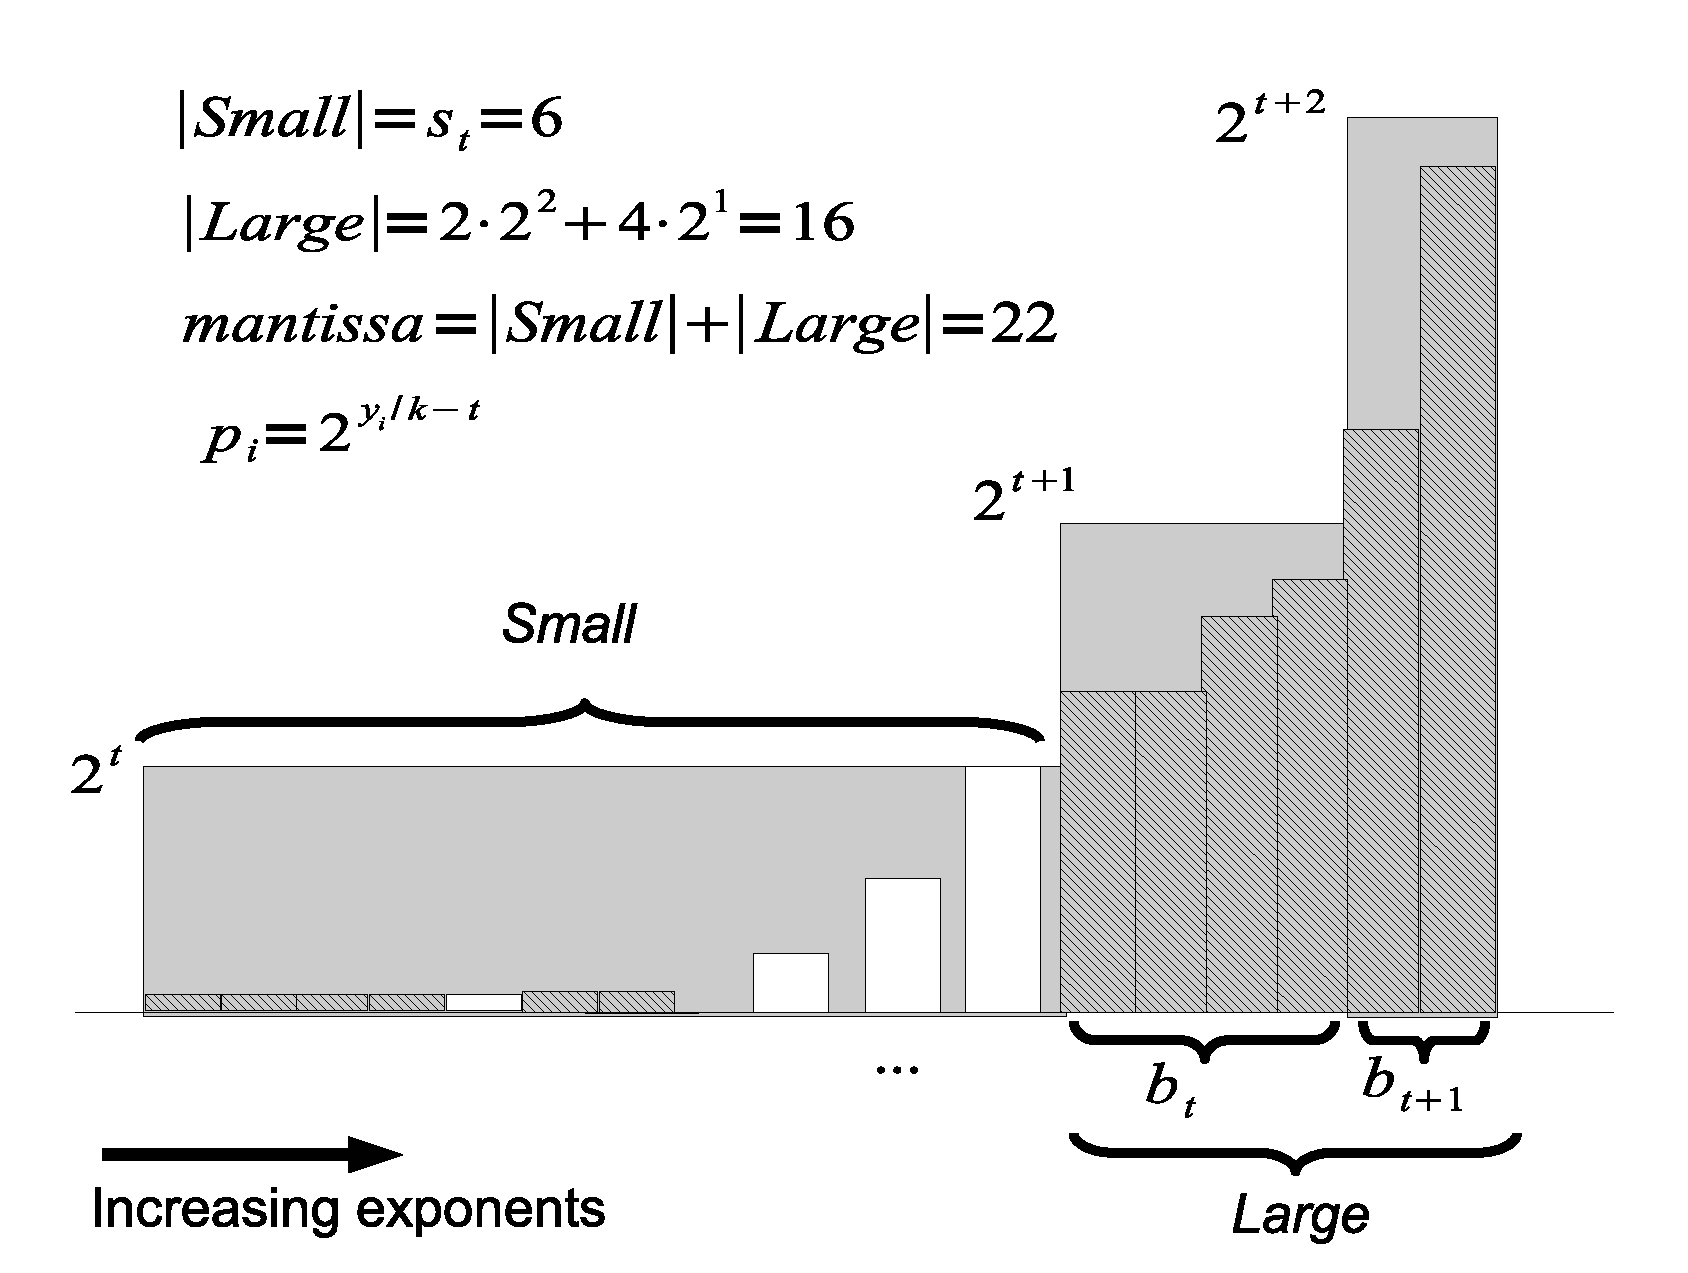
\includegraphics[width=6in]{fullScheme.eps}
\caption{The full sampler scheme.  The entire gray shaded area indicates the
  weight that is included in the mantissa. True
  item weights are represented by hatched bars, and the probability of
  rejection  consists of all solid gray regions.} 
\label{fig:fullScheme}
\end{figure}

To calculate the norm, we first calculate the mantissa. We consider all 
bucket exponents relative to $t$ rather than to $0$; for example,
all item weights in \smallset are counted as $2^0=1$, all item weights in the
bucket with exponent $t+1$ are counted as $2^1=2$, etc. This technique 
ensures an upper bound of $4n$ on the mantissa value (see
Appendix~\ref{sec:normProof} for details),  which implies that the mantissa 
can be stored accurately as a 64-bit integer as
long as $ n < 2^{62}$. This is significantly larger than any problem size
would require in the foreseeable future.  We return the (mantissa, $t$) pair 
as the sampler norm.

When sampling, we consider the total weight in the sampler to consist only of 
the mantissa, and we consider all item exponents relative to $t$.  
Note that because \smallset can contain items with arbitrarily small
weights relative to $2^t$, the probability of rejection in \smallset could be 
arbitrarily high. However, since \largeset contains $\ge 1/2$ the total weight 
and the  probability of rejection in \largeset is $\le 1/2$, then the overall 
probability of rejection in the sampler is $\le 1/4$, which is essential for
 satisfying the performance requirement specified in our discussion of the 
interface.  

By our choice of $t$, \largeset is guaranteed to contain 
$\le \log n$ buckets. It is this structural feature which produces the
worst-case time bound on all sampler operations. Constant time per operation
is achieved if a constant fraction of the
weight in a sampler is contained in its first $O(1)$ buckets. In 
practice, we find this condition to hold for a variety of problem inputs.

The dense clustering of items in the first few buckets in practice motivates our
deviation from the theoretical data structures of \cite{hagerup1993} and
\cite{matias1993}. We group items into buckets much as in these structures,
but they 
impose an additional recursive hierarchy onto the buckets.  
Such a hierarchy guarantees good
worst-case performance, since sampler operations can drill down through the 
hierarchy to a bucket rather than linearly traversing all buckets as our
sampler does.  However, drilling down through a bucket hierarchy also 
introduces overhead into each
sampler operation.  Since the weight of the samplers is densely
concentrated into just a few buckets in our application, we find that the 
overhead incurred by a recursive bucket structure is more expensive than a 
linear-traversal scheme.

\section{Sampling operations} \label{sec:samplerOps}
We now discuss the probabilistic sampling operations used in the fastpc algorithm and show that these operations can be performed with small bounded precision loss.

%% Q: Where do we use RANDMAX?  Do I have the sampling procedure correct?

Two sampling operations are required by the fastpc algorithm: sampling uniformly from the unit range [0,1] in lines ??? of fastpc and choosing an item from a sampler with probability proportional to its weight (which is the goal of the random-pair() subroutine).  This second operation is accomplished simply by invoking the \func{sample()} function of the appropriate samplers, the mechanics of which is described in the previous section.

  %% Coin-flipping trick
Lines ??? of fastpc require a uniform random sample in the range [0,1] and a comparison of the quantities $M_{ij'}\incVal$ and $M_{i'j}\incVal$ to that sampled value.
Because these quantities could be arbitrarily small, the granularity of a given machine's built-in sampling procedure may not be sufficient to ensure a fair sample and comparison.  
We therefore use a custom sampling procedure similar in spirit to the bucket-selection procedure of the \func{sample()} function when the value of either of these quantities is $< 1/2$.  When a quantity is $>= 1/2$, we simply use the machine's built-in random sampling procedure and perform the comparison in a straightforward way.
We describe the procedure for the comparison test when $M_{ij'}\incVal < 1/2$, and note that the test for $M_{i'j}\incVal$ is identical.
Conceptually, this sampling procedure divides the [0,1] interval into smaller intervals with boundaries determined by successive powers of $1/2$.  
We then iteratively select an interval by repeatedly sampling in [0,1] uniformly and moving to the next interval only if the sampled value is $> 1/2$.  
If the selected interval's lower boundary is greater than $M_{ij'}\incVal$, then the procedure terminates and returns that $M_{ij'}\incVal$ is smaller than the sampled value. 
Similarly, if during the iteration process the current interval's upper boundary is smaller than $M_{ij'}\incVal$, then the procedure terminates and returns that $M_{ij'}\incVal$ is greater than the sampled value.  
If $M_{ij'}\incVal$ lies between the boundaries of the selected interval, we normalize that interval to the [0,1] interval, adjusting $M_{ij'}\incVal$ accordingly, and recursively repeat the procedure.
The probability of reaching any interval diminishes exponentially with the size of the interval, and so this procedure is expected to terminate in a constant number of iterations w.h.p.

We now show that the overall impact of these approximate sampling operations on the solution generated by fastpc is less than a $\epsUp$-factor.  

%% What to say about RANDMAX?
   
To analyze the impact of the random-pair() subroutine using our \func{sample()} function on the overall modified algorithm, we consider the probability $\gamma_{ij} $ of returning a particular $(i,j)$ pair in an exact-arithmetic model and the probability $\gamma_{ij}'$ of returning the corresponding $(i,j)$ pair in our computational model using the rejection method.
We first note that the weight $w'(sampler)$ of any sampler in our regime could differ from its weight $w(sampler)$ in the exact-arithmetic regime by at most a factor of $\epsUp$.  
We next observe that since the entire random-pair() procedure is restarted upon rejection, $\gamma_{ij} '$ does not depend on any rejections that may occur during a call to random-pair() and can be calculated as though no rejections happen.  
Therefore, $\gamma_{ij}'$ is proportional to $w'(i)/w'(sampler)$ and $w'(j)/w'(sampler)$.
Now, since the weight of any individual item $w'(i)$ (or, equivalently, $w'(j)$) in our modified samplers also differs from its weight $w(i)$ in the exact regime by at most a factor of $\epsUp$, then the ratios of their weights clearly also differ by at most a $\epsUp$ factor.  
This implies that $\gamma_{ij} ' \le \epsUp \gamma$. 

% Outline
% 1. Show that necessary core lemmas are satisfied (w/additional small error)
% 2. Error incurred by sampling
%   -- analysis of random-pair() -- should only affect E(selecting particular $i, j$)
%      -- 3 steps: a) rejection method: lose $\epsUp$-factor in norms
%                         b) justification of analyzing prob of selecting particular $i,j$ given that we don't reject (i.e., can ignore any bias in the choice of distros)
%                         c) ratio argument for not being more than $\epsUp$ off from selection using exact rejection strategy
% 3. Sampling: how to sample in $\left[ 0, 1 \right]$ and $\left[ 1, 2 \right]$
%   -- coin-flipping trick for values $\le 1/2$ 
 %  -- precision issues / RANDMAX ?
   
   \section{Modified FASTPC algorithm} \label{sec:mod-fastpc}
To accommodate our arithmetic model and our sampling implementation, we introduce the following changes to the fastpc algorithm:

% Q: do we need to list the changes that have already been described?  
% Pro: see them all in the same place.
% Con: redundant.

\begin{enumerate}
% Already described when introducing arithmetic model
\item We replace the value of $\epsilon$ given as a problem parameter with a new $\epsilon$ that 
 satisfies $(1+\epsilon)^k = 2$ for some integer $k$.  

% Already described when introducing arithmetic model
\item Instead of maintaining $\phat_j$ as $(1-\epsilon)^{\yhat_j}$, we maintain it as $\epsUp^{-\yhat_j}$.  

% Already described in sampler section
\item We modify the sampling procedure presented in fastpc; details are given in Section~
\ref{sec:sampler}.

\item We change line ??? of fastpc so that $y_i$ and its 
samplers are only updated if $\epsDown M_{ij'}\incVal \geq z$.
This implies that $E[\Delta y] = \epsDown E[\Delta Mx] 
= \epsDown \alpha M \phat / \sizeof{\phat}$. We calculate
$\yhat$ as in \cite{kouf2007}, so that 
$E[\Delta \yhat] = E[\Delta M^T \xhat] = \alpha M^T p / \sizeof{p}$.  

With this modification, the analysis of correctness and running time from
\cite{kouf2007} still holds, with an additional additive $\epsilon$-error in 
the approximation guarantee.  Details are given in Section~\ref{sec:analysis}.

\end{enumerate}

% Outline
%1. Introduce modified $\epsilon$ such that $(1+\epsilon)^k = 2$
%2. Introduce $\epsDown$
%3. Introduce new $\epsDown$-adjustment to update step
%4. Introduce probability of rejection.
%


\section{Analysis of modified FASTPC} \label{sec:analysis}

% Outline
% Use some bound in terms of $\epsUp$, but based on $1 + 1/RANDMAX$, so that analysis is convenient but we don't lose more than a $\epsUp$ factor overall due to precision issues 

We now follow the analysis in \cite{kouf2007}, Lemmas 3 and 4, to show that with
probability at least $1-\frac{3}{rc}$ the
revised algorithm returns a feasible $(1-O(\epsilon))$-approximate solution.
 We use the same potential function as in \cite{kouf2007}, namely 
$\Phi = \sizeof{p} \sizeof{\phat}$.  We first show that it is a
super-Martingale. If $p'$ and $\phat '$ denote $p$ and $\phat$ after a given
round of the main loop of the algorithm, then 
\begin{align*}
\sizeof{p '} &= \sum_i p_i(1+\epsilon)^{\Delta y_i} \\
 &= \sum_i p_i(1+\epsilon \Delta y_i) \\
 &= \sizeof{p} + \epsilon p ^T \Delta y.\\
\text{Also,  } \sizeof{\phat'} &= \sum_j \phat_j(1+\epsilon)^{-\Delta \yhat_j} 
\\ &= \sum_j \phat_j(1-\frac{\epsilon}{1+\epsilon})^{\Delta \yhat_j} 
\text{  since  }
\frac{1}{1+\epsilon} = 1 - \frac{\epsilon}{1+\epsilon} \\
 &=\sum_j \phat_j(1-\frac{\epsilon}{1+\epsilon} \Delta \yhat_j) \\
 &=\sizeof{\phat} - \frac{\epsilon}{1+\epsilon} \phat^T \Delta \yhat. 
\end{align*}
Multiplying these equations gives
\begin{align*}
\Phi ' = \sizeof{p'} \sizeof{\phat '} \leq \sizeof{p} \sizeof{\phat} + 
\epsilon \sizeof{\phat} p^T \Delta y - \frac{\epsilon}{1+\epsilon} 
\sizeof{p} \phat ^T \Delta \yhat.
\end{align*}
Taking expectations and substituting for $E[\Delta y]$ and $E[\Delta \yhat]$ 
gives
 \begin{align*}
\sizeof{p'} \sizeof{\phat '} &\leq \sizeof{p} \sizeof{\phat} + 
\frac{\epsilon \epsDown
\sizeof{\phat} p^T \alpha M \phat}{\sizeof{\phat}} - 
\frac{\epsilon \sizeof{p} \phat ^T \alpha M^T p}
{(1+\epsilon) \sizeof{p}}\\
&= \sizeof{p} \sizeof{\phat} + 
 \epsilon \epsDown \alpha  p^T  M \phat -
\frac{\epsilon}{1+\epsilon} \alpha \phat ^T  M^T p \\
&= \sizeof{p} \sizeof{\phat} 
\end{align*}

By Wald's equation $E[\Phi]$ when the algorithm terminates is at most its 
initial
value $rc$.  Applying the Markov bound, with probability at least
$1-\frac{1}{rc}$, at termination $\max_i p_i \max_j \phat _j \leq 
\sizeof{p} \sizeof{\phat} \leq (rc)^2$.  By the argument in \cite{kouf2007}, 
then, Lemma 3 holds, i.e. $max_i y_i \leq N$ and 
$min_j \yhat _j \geq N(1-2\epsilon)$. 

Lemma 4 shows that $y \approx Mx$ and $\yhat \approx M^T\xhat$.  Since we have
introduced an $O(\epsilon)$-factor adjustment to $y$, this is where we
incur an extra $\epsilon$-factor in the performance guarantee. To prove the
lemma we use the Chernoff bound for random stopping times given in
Lemma 10.

% Q: What is exact approximation guarantee now?  How does RANDMAX fit in?
For part (1) we substitute $\Delta (\epsDown)M_i x$ for $x_t$ and 
$\Delta y_i$ for $y_t$ in Lemma 10.  The proof holds as in \cite{kouf2007}, with the conclusion that with probability at least $1-\frac{3}{rc}$, 
$\frac{\sizeof{x^*}}{\sizeof{\xhat ^*}} = \frac{\min_jM_J^T\xhat}{\max_iM_ix}
\geq 1-???\epsilon$. 

\section{Conclusions and future work} \label{sec:conclusion} 

\section{Appendix}
\subsection{Upper Bound on Sampler Norm}\label{sec:normProof}
Because of the way item weights are calculated internally, the sampler norm can be
upper-bounded by $4n$, where $n$ is the number of items
in the sampler.  Without loss of generality, we show this by induction for the
sampler $p$.  First note that if $t$ were equal to
the maximum
exponent of any item in $p$, then all items would be in \smallset
and $\sizeof{p}$, the norm of $p$, would be $n$.  Now given any value of
$t$, consider decrementing
$t$ by $k$ to $t'$, which transfers one bucket from \smallset to \largeset.
Let  $s_{t}$ be the number of items in \smallset relative to $t$,
and likewise for $s_{t'}$. Let $\sizeof{p}'$ be the norm of $p$ calculated
using $t'$ as the base exponent. Then we know that 
$\sizeof{p}' \le 2 \cdot \sizeof{p}$, since moving $t$ by $k$ doubles the
weights of all items in \largeset and at most doubles the weight of any
item in \smallset by adding it to \largeset.  But by our calculation of
$t$, it must be the case that $\sizeof{p} \le 2 \cdot s_{t}$, else we
would have already found the final value of $t$ and would not need to
decrement it further.  Clearly $s_{t} \le n$, and so we have that 
$\sizeof{p}' \le 4 \cdot s_{t} \le 4 \cdot n$.  


%%%%%%%%%%%%%%%%%%%%%%%%%%%%
%%		Master's writeup
%%
%%%%%%%%%%%%%%%%%%%%%%%%%%%%

%\section{Introduction} \label{sec:intro}
%In \cite{kouf2007}, Koufogiannakis and Young give a randomized algorithm for 
%solving pure packing and covering linear programs.  Here, a packing problem is 
%of the form $\max\{a \cdot x : Mx \le b, x \ge 0\}$, and a covering problem is 
%of the form $\min\{a \cdot \xhat : M \xhat \ge b, \xhat \ge 0\}$, where
%the entries in the constraint matrix $M$ are non-negative.  
%They build on an algorithm by 
%Grigoriadis and Khachiyan \cite{grigoriadis1995} to simultaneously build up 
%primal 
%and dual solutions until a $(1 \pm O(\epsilon))$ ratio exists between them, 
%which by weak duality implies $(1 \pm O(\epsilon))$-approximate solutions. 
%The primal 
%and dual solution vectors are initialized to zero and then are built up in a 
%series of rounds. In each round, one primal and one dual variable are 
%simultaneously chosen and incremented by a small amount. 
%The primal variable is chosen from a distribution determined by the current 
%dual solution vector, and vice versa.
%The authors show that their algorithm returns a 
%$(1 \pm O(\epsilon))$-approximate solution in running time $\runtime$ 
% with high probability.  We assume a high degree of familiarity with this
% algorithm, which we refer to as ``fastpc,'' in the current work.
%
%The fastpc algorithm has proved non-trivial to implement.  
%Koufogiannakis and Young 
%implemented the algorithm in C++ for the restricted case of 0/1 
%input matrices, and their results confirm asymptotic superiority to the 
%Simplex algorithm as implemented in the Gnu Linear Programming Kit (GLPK).  
%We present a generalized implementation for input matrices with coefficients 
%in $[0, \infty)$.  As suggested in \cite{kouf2007}, this is primarily 
%accomplished by employing the non-uniform-increments scheme of Garg and 
%Konemann \cite{garg1998} and by maintaining approximate, rather than exact, 
%constraint values.  
%In the following sections, we present the challenges of implementing the 
%generalized algorithm, relevant previous
% approaches to these challenges, and our own design decisions. 
%
%\section{Implementation Requirements} \label{sec:requirements}
%The complexity of implementing fastpc lies primarily in maintaining the
%dynamic 
%probability pseudo-distributions $p$, $\phat$, $\pXuh$, and $\phXu$ (a 
%pseudo-distribution is a vector of probability values that do not add
%up to one, i.e. they have not been normalized).  We implement a data structure
%called a ``sampler'' for this purpose, drawing heavily on the schemes for 
%theoretical data structures previously proposed  by Hagerup et al. in 
%\cite{hagerup1993} and Matias et al. in \cite{matias1993}. Specifically, we
%employ the rejection method when sampling and the clustering of items with
%similar weights into buckets.  
%
%Item weights as given in fastpc are powers of $(1+\epsilon)$ for
%items in $p$ and $\pXuh$, and powers of $(1-\epsilon)$
%for items in $\phat$ and $\phXu$.  We modify
%this scheme by rounding $\epsilon$ to satisfy $(1+\epsilon) = 2^{1/k}$ for 
%some integer $k$. Then items in all samplers are maintained as powers of 
%$(2^{1/k})$, with exponents in $\phat$ and
%$\phXu$ being nonpositive and decreasing.  We show how to compensate for this 
%change in Section~\ref{sec:revisedAlg}.  To simplify sampler operations and 
%help prevent precision loss, we store all item weights by their exponent only.  
%
%The sampler provides the following interface to fastpc: 
%\begin{enumerate}
%\item \func{create\_sampler(}\args{int $n$, int[] expts}\func{):} create 
%  sampler containing $n$ items with initial exponents from
%  \args{expts}.
%
%\item \func{sample(}\args{sampler $s$}\func{):} return some $s_i$ or
%  $\reject$.  Each item is chosen with probability
%    proportional to its weight; the sampler returns $\reject$ with some
%    probability according to the rejection method.
%
%\item \func{norm(}\args{sampler $s$}\func{):} return total
%  weight contained in $s$, including the weight associated with rejection, as a
%  (mantissa, exponent) pair. Because the total
%    weight in a sampler can exceed the storage capacity of a standard
%    double-precision word, which includes 11 bits for the exponent, we
%    simulate floating-point words by storing a mantissa and exponent in
%    separate words, allowing 32 or 64 bits of storage for the exponent.
%
%\item \func{increment\_exponent(}\args{sampler $s$, int
%    $i$}\func{)};
%    \func{decrement\_exponent(}\args{sampler $s$, int
%    $i$}\func{):} increase/decrease exponent of $s_i$ by 1.  
%
%\item \func{remove(}\args{sampler $s$, int $i$}\func{):} remove $s_i$ from
%  $s$. 
%  
%\end{enumerate}
%
%In order to meet the runtime guarantee of fastpc, all sampler operations must
%be performed in amortized $O(1)$ time.  In addition, the probability of a
%\func{sample()} call returning $\reject$ must be constant and $< 1$.  In section \ref{sec:fullScheme} we show a
%worst-case running time of $O(\log n)$ per operation, but an empirically 
%observed time of $O(1)$.
%
%\section{Sampler} \label{sec:sampler}
%We present our sampling data structure in three stages: first
%for the special case where all item weights are whole powers of $2$, then
%for arbitrary item weights but with no runtime guarantee, and finally for
%arbitrary item weights with an amortized  $\log n$ runtime guarantee per 
%operation.
%
%\subsection{Special Case: Whole Powers of Two} \label{sec:specialCase}
%We first present a sampler suited to handle item weights that are whole powers 
%of $2$.  This is the special case in which the probability of rejection is
%$0$.
%
%For each exponent whose value is held by at least one item, we maintain a
%bucket 
%of all items currently having that exponent.  To calculate the norm, we
%multiply the number of items in each bucket by the
%appropriate power of $2$ and sum the results.  To sample, we first choose a
%random integer between $0$ and the norm of the
%sampler. We then scan through the buckets from largest exponent to smallest
%until the cumulative weight of the scanned buckets exceeds the random integer.
%Finally, we choose an item uniformly from the last bucket scanned and return it.
%To increment (decrement) an
%item's exponent, we remove the item from the bucket of its old exponent and add
%it to the bucket of its new exponent.
%
%%We then scan through the buckets, beginning with
%%the largest one. If the total weight of all items in that bucket is larger
%%than $w$, we uniformly sample one of these items and return it.  If not, then
%%we subtract the weight in the first bucket from $w$ and consider the
%%next-largest bucket in the same way.  
%
%%This structure is shown in 
%%Figure~\ref{fig:wholePow}.
%
%%\begin{figure}[ht]
%%\centering
%%\includegraphics[width=6in]{paper-wholePow}
%%\caption{A sampler for $p$, with items shown as hatched bars with areas
%%  proportional to their weights. White bars
%%  indicating nonexistant buckets are shown as placeholders. The calculation of
%%  the norm of $p$ is shown. }
%%\label{fig:wholePow}
%%\end{figure}
%
%\subsection{General Case} \label{sec:generalCase}
%We next describe a sampler suited to handle arbitrary item weights.  Our 
%strategy will be to consider all item weights to be their next-highest power of
%$2$ and use the rejection method to account for their actual
%weights.  
%
%We calculate the sampler norm exactly as in the previous scheme.
%Note that the norm could now be larger than the sum of 
%all item weights; the difference between the two is the probability of 
%rejection.
%We sample as in the previous scheme, with the addition of a rejection step.  
%Once we have chosen an item, we accept and return it 
%with probability equal to its weight over the next-highest power of two.  
%This quantity is $\ge 1/2$.  If we do not accept the chosen item, we return 
%$\reject$. To increment (decrement) an item's exponent, we increment 
%(decrement) its stored exponent and move it to a new bucket if necessary.
%
%%The overall sampler structure is shown in Figure~\ref{fig:fracPow}.
%
%%\begin{figure}[ht]
%%\centering
%%\includegraphics[width=6in]{paper-fracPow}
%%\caption{A sampler for $p$ where an item can have arbitrary weight.  Items in
%%  large buckets are shown as hatched bars with sizes proportional to their 
%%weights, and $\reject$ consists of all solid gray regions.   }
%%\label{fig:fracPow}
%%\end{figure}
%
%\subsection{Full Scheme} \label{sec:fullScheme}
%We now introduce a modification to the previous data structure that both 
%ensures correctness and gives a $\log n$ worst-case running time guarantee.  
%%%%%%%%%%%%%%%%%%%%%%%%%%%
%%We introduce a few techniques to prevent these potential problems. We first
%%address the potential overflow in sampler norms.
%%When sampling, instead of using a sampler's full norm, we calculate a
%%normalized upper bound on the norm as follows.  
%We first calculate a certain threshold exponent $t$.  We consider all
%items with exponent less than $t$ to be in a single bucket which we call
%\smallset, and we refer to all other items collectively as \largeset. We
%set $t$ to be the highest exponent such that the total weight in
%\largeset is at least the total weight in \smallset.  In other words, we
%set $t$ such that at least half the sampler's total weight is in \largeset.  
%An illustration of the full sampler is shown in Figure~\ref{fig:fullScheme}.
%
%\begin{figure}[ht]
%\centering
%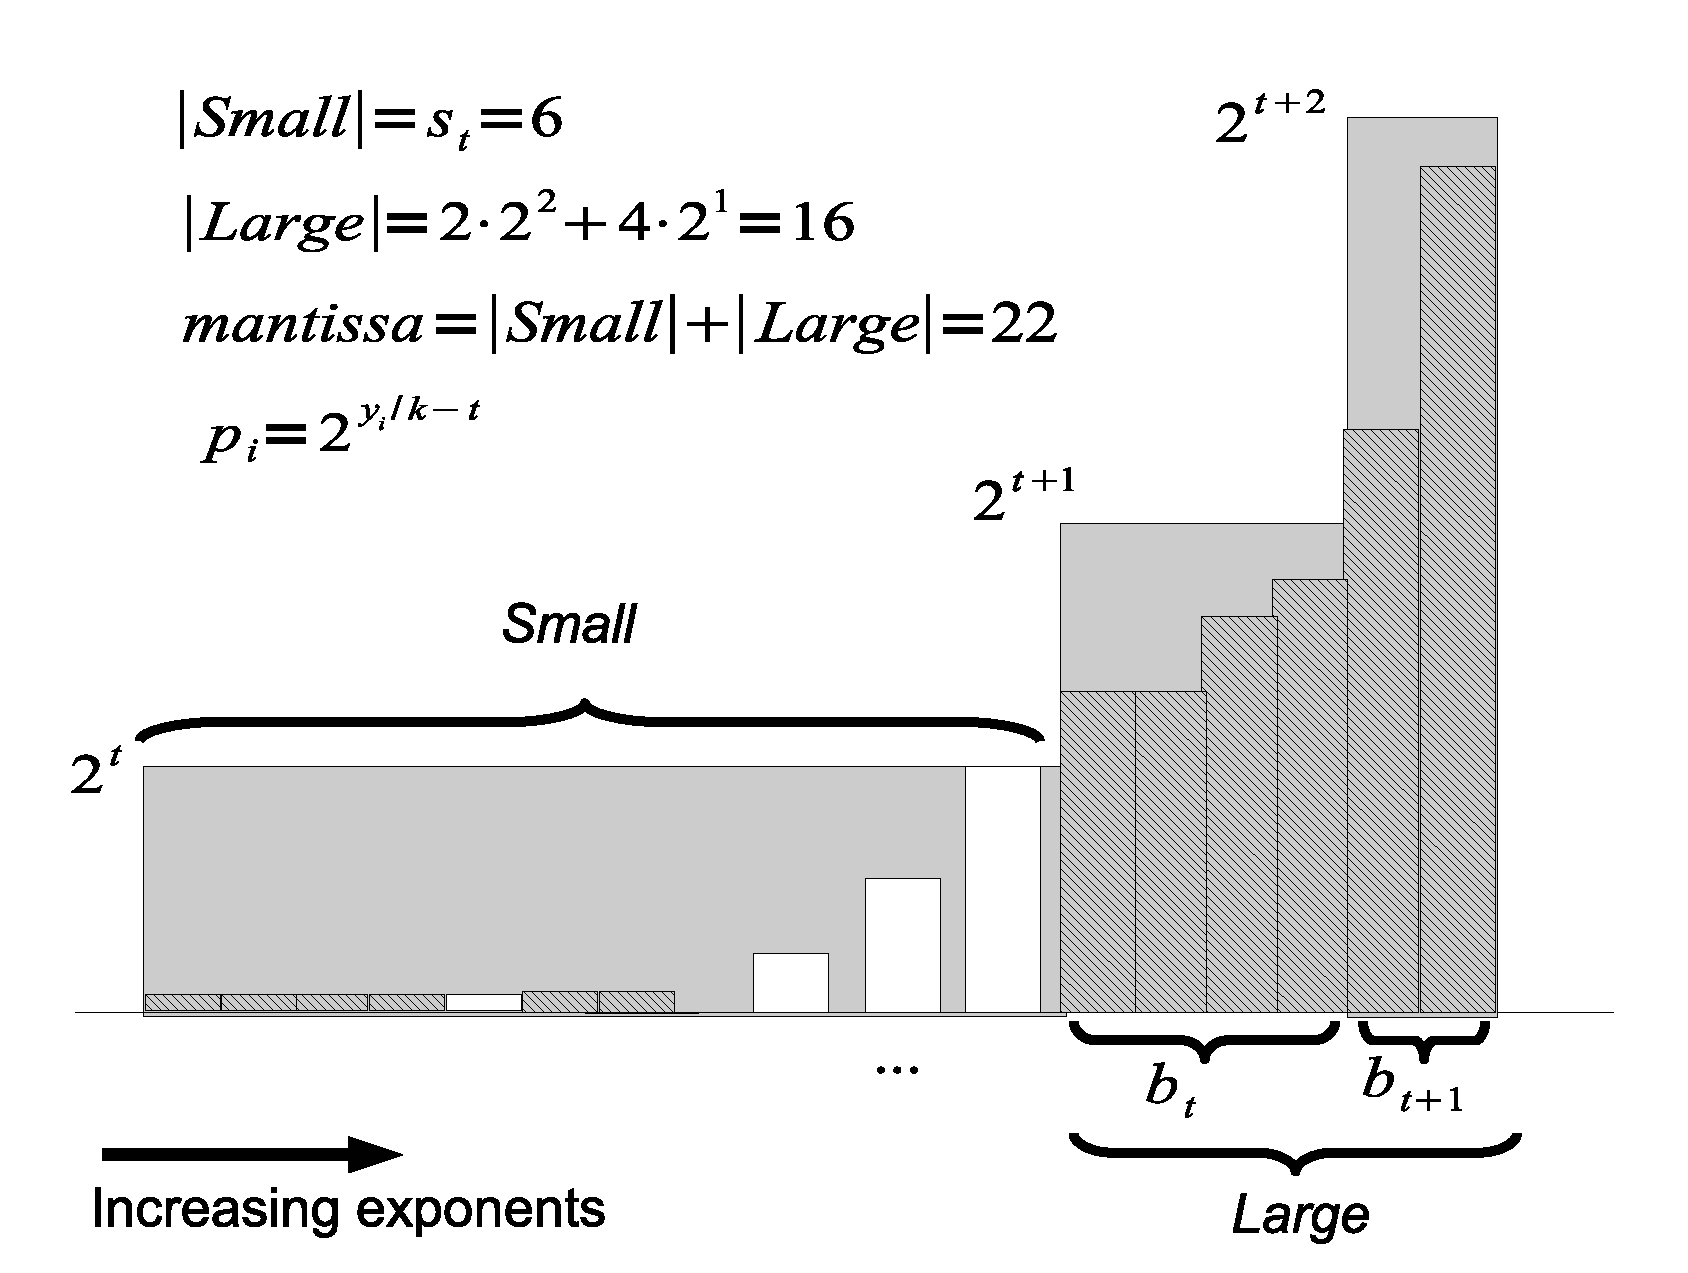
\includegraphics[width=6in]{fullScheme.eps}
%\caption{The full sampler scheme.  The entire gray shaded area indicates the
%  weight that is included in the mantissa. True
%  item weights are represented by hatched bars, and the probability of
%  rejection  consists of all solid gray regions.} 
%\label{fig:fullScheme}
%\end{figure}
%
%To calculate the norm, we first calculate the mantissa. We consider all 
%bucket exponents relative to $t$ rather than to $0$; for example,
%all item weights in \smallset are counted as $2^0=1$, all item weights in the
%bucket with exponent $t+1$ are counted as $2^1=2$, etc. This technique 
%ensures an upper bound of $4n$ on the mantissa value (see
%Appendix~\ref{sec:normProof} for details),  which implies that the mantissa 
%can be stored accurately as a 64-bit integer as
%long as $ n < 2^{62}$. This is significantly larger than any problem size
%would require in the foreseeable future.  We return the (mantissa, $t$) pair 
%as the sampler norm.
%
%When sampling, we consider the total weight in the sampler to consist only of 
%the mantissa, and we consider all item exponents relative to $t$.  
%Note that because \smallset can contain items with arbitrarily small
%weights relative to $2^t$, the probability of rejection in \smallset could be 
%arbitrarily high. However, since \largeset contains $\ge 1/2$ the total weight 
%and the  probability of rejection in \largeset is $\le 1/2$, then the overall 
%probability of rejection in the sampler is $\le 1/4$, which is essential for
% satisfying the performance requirement specified in our discussion of the 
%interface.  
%
%Because of the way $t$ is chosen, \largeset is guaranteed to contain 
%$\le \log n$ buckets. It is this structural feature which produces the
%worst-case time bound on all sampler operations. Constant time per operation
%is achieved if a constant fraction of the
%weight in a sampler is contained in its first $O(1)$ buckets. In 
%practice, we find this condition to hold for a variety of problem inputs.
%
%%% Keep the following?
%%From the standpoint of the operation of fastpc, this assumption makes sense.  
%%As the algorithm progresses, we expect $\approx n$ constraints to be ``close'' 
%%to their final value, in which case their corresponding items' exponents will be
%%close together.  In practice, we also find this assumption to hold for a
%%variety of problem inputs; in fact, we find that more than $90\%$ of the
%%weight of a sampler is often contained in the first $5$ buckets.
%
%The dense clustering of items in the first few buckets in practice motivates our
%deviation from the theoretical data structures of \cite{hagerup1993} and
%\cite{matias1993}. We group items into buckets much as in these structures,
%but they 
%impose an additional recursive hierarchy onto the buckets.  
%Such a hierarchy guarantees good
%worst-case performance, since sampler operations can drill down through the 
%hierarchy to a bucket rather than linearly traversing all buckets as our
%sampler does.  However, drilling down through a bucket hierarchy also 
%introduces overhead into each
%sampler operation.  Since the weight of the samplers is densely
%concentrated into just a few buckets in our application, we find that the 
%overhead incurred by a recursive bucket structure is more expensive than a 
%linear-traversal scheme.
%
%\section{Revised Algorithm}\label{sec:revisedAlg}
%We now describe two modifications to the fastpc algorithm necessitated by our
%sampler. The first
%accounts for the new definitions of $\phat$ and $\phXu$.
%We change line 8 of fastpc so that $y_i$ and its 
%samplers are only updated if $(1-\epsilon)M_{ij'}\delta_{i'j'} \geq z$.
%This implies that $E[\Delta y] = (1-\epsilon) E[\Delta Mx] 
%= (1-\epsilon)\alpha M \phat / \sizeof{\phat}$. We calculate
%$\yhat$ as in \cite{kouf2007}, so that 
%$E[\Delta \yhat] = E[\Delta M^T \xhat] = \alpha M^T p / \sizeof{p}$.  
%
%With this modification, the analysis of correctness and running time from
%\cite{kouf2007} still holds, with an additional additive $\epsilon$-error in 
%the approximation guarantee.  Details are given in Appendix~\ref{sec:analysis}.
%
%The second modification accounts for the possibility of returning $\reject$ when
%sampling.  Since the probability of rejection is included in the sampler
%norms, and the sampling process in fastpc begins with a calculation in the
%\func{random-pair()} function based on the norms, we restart the entire sampling
%process whenever $\reject$ is returned.  Because the probability of
%returning $\reject$ is constant and $< 1$, the modified algorithm is still 
%guaranteed to make progress at a rate within a constant factor of the original
%algorithm.   
%
%\section{Conclusion} \label{sec:conclusion}
%We have introduced the requirements for a sampling data structure as
%needed by the fastpc algorithm, and introduced a 
%structure that meets those requirements.  In the future we hope to introduce
%optimizations to this data structure to improve its expected running time, as
%well as further study its performance on different types of inputs.
%
%\section{Appendix}
%\subsection{Upper Bound on Sampler Norm}\label{sec:normProof}
%Because of the way item weights are calculated internally, the sampler norm can be
%upper-bounded by $4n$, where $n$ is the number of items
%in the sampler.  Without loss of generality, we show this by induction for the
%sampler $p$.  First note that if $t$ were equal to
%the maximum
%exponent of any item in $p$, then all items would be in \smallset
%and $\sizeof{p}$, the norm of $p$, would be $n$.  Now given any value of
%$t$, consider decrementing
%$t$ by $k$ to $t'$, which transfers one bucket from \smallset to \largeset.
%Let  $s_{t}$ be the number of items in \smallset relative to $t$,
%and likewise for $s_{t'}$. Let $\sizeof{p}'$ be the norm of $p$ calculated
%using $t'$ as the base exponent. Then we know that 
%$\sizeof{p}' \le 2 \cdot \sizeof{p}$, since moving $t$ by $k$ doubles the
%weights of all items in \largeset and at most doubles the weight of any
%item in \smallset by adding it to \largeset.  But by our calculation of
%$t$, it must be the case that $\sizeof{p} \le 2 \cdot s_{t}$, else we
%would have already found the final value of $t$ and would not need to
%decrement it further.  Clearly $s_{t} \le n$, and so we have that 
%$\sizeof{p}' \le 4 \cdot s_{t} \le 4 \cdot n$.  
%
%\subsection{A Counterexample To Rounding}\label{sec:counterexample}
% We have described a sampler that carefully maintains the exponents of all 
%items and,  using the rejection method, accounts for all weights when sampling. 
%At first, this may seem like overkill.  Since the fastpc algorithm can 
%tolerate a small perturbation of the probability distributions 
%(on the order of $(1 \pm \epsilon)$-factor perturbations), and since any item
% with weight exponentially smaller than another item will be extremely unlikely to be chosen in any sampling step, it would seem that we could round ``tiny''
% weights down to 0 when sampling and maintain correctness.  However, this is 
%not the case.  
%In \cite{kouf2007}, the authors allude to a procedure originally described by Luby and Nisan in \cite{luby1993} by which matrix coefficients can be put in a bounded range at the cost of an $\epsilon$-factor in the approximation guarantee. 
%Assuming that this scheme is employed, the maximum possible coefficient 
%(and therefore the maximum initial element in $\pXuh$ or $\phXu$) is no more
% than $n^2/\epsilon^2$ times the minimum element.  
%Even with so large a difference
% in sampler weights as this, rounding the smallest weights to 0 still
% invalidates 
%the proof of correctness for fastpc, as the following example shows. 
%Consider a constraint matrix $M$ of the following form:
%$\begin{pmatrix}
%1&\ldots&1&\frac{m^2}{\epsilon^2}\\
%1&\ddots&&1\\
%\vdots&&&\vdots\\
%1&\ldots&&1
%\end{pmatrix}$
%
%Assume the matrix has $m$ rows and $m$ columns, with $m$ large and $\epsilon$
%small. At the start of fastpc, the distributions and increment matrix have the
%following forms:\\
%\begin{center}
%\begin{tabular}{rl}
%$p = \left( 1,\ldots,1 \right)$ &
%$\pXuh = \left( \frac{m^2}{\epsilon^2},1,\ldots,1 \right)$\\
%$\phat = \left( 1,\ldots,1 \right)$&
%$\phXu = \left( 1,\ldots,1,\frac{m^2}{\epsilon^2} \right)$
%\end{tabular}
%\\
%$\delta = \begin{pmatrix}
%\frac{1}{1+m^2/\epsilon^2}&\ldots&\frac{1}{1+m^2/\epsilon^2}&
%\frac{1}{2m^2/\epsilon^2}\\
%\frac{1}{2}&\ldots&\frac{1}{2}&\frac{1}{1+m^2/\epsilon^2}\\
%\vdots&\ddots&&\vdots\\
%\frac{1}{2}&\ldots&\frac{1}{2}&\frac{1}{1+m^2/\epsilon^2}
%\end{pmatrix}$
%\\
%\end{center}
%
%According to the calculation in the random-pair() function, with probability
%$1/2$ a sample will be chosen from the pseudo-distributions $p$ and $\phXu$.
%Assume this happens.  We will analyze the expected change in a particular
%dual variable $\xhat_2$.
%\begin{align*}
%E[\Delta \xhat_2] &= (\text{chance of selecting } \xhat_2) \times
%                    (\text{increment for chosen pair}) \\
%&= \sum_j \text{chance of selecting } (\xhat_2,x_j) \cdot \delta_{2,j} \\
%&\approx \frac{1}{m} \left[ \frac{\epsilon^2}{m+\epsilon^2}(\frac{1}{2})
%                      + (1-\frac{\epsilon^2}{m+\epsilon^2}) 
%                      (\frac{1}{1+m^2/\epsilon^2}) \right] = 
%O(\epsilon^2/m^2) \\
%&\phantom{\approx}\text{Here the leftmost term inside the brackets represents}\\
%&\phantom{\approx}\text{the sum of all columns except column } m, \\
%&\phantom{\approx}\text{and the rightmost term represents column } m.
%\end{align*} 
%
%If we round all weights of $1$ down to $0$, the expected change in $\xhat_2$
%would be calculated as follows:
%\begin{align*}
%E[\Delta \xhat_2] &\approx \frac{1}{m} \left[ 0(\frac{1}{2})
%                      + 1(\frac{1}{1+m^2/\epsilon^2}) \right] = 
%O(\epsilon^2/m^3)
%\end{align*} 
%
%The difference between these two quantities is significant.  Since the expected change in variables differs significantly
%from what is needed by our current analysis to show the correctness of fastpc 
%with constant probability, 
%this is a valid counterexample to the technique of rounding to $0$.  
%
%\subsection{Analysis of Revised Algorithm} \label{sec:analysis}
%We now follow the analysis in \cite{kouf2007}, Lemmas 3 and 4, to show that with
%probability at least $1-\frac{3}{rc}$ the
%revised algorithm returns a feasible $(1-O(\epsilon))$-approximate solution.
% We use the same potential function as in \cite{kouf2007}, namely 
%$\Phi = \sizeof{p} \sizeof{\phat}$.  We first show that it is a
%super-Martingale. If $p'$ and $\phat '$ denote $p$ and $\phat$ after a given
%round of the main loop of the algorithm, then 
%\begin{align*}
%\sizeof{p '} &= \sum_i p_i(1+\epsilon)^{\Delta y_i} \\
% &= \sum_i p_i(1+\epsilon \Delta y_i) \\
% &= \sizeof{p} + \epsilon p ^T \Delta y.\\
%\text{Also,  } \sizeof{\phat'} &= \sum_j \phat_j(1+\epsilon)^{-\Delta \yhat_j} 
%\\ &= \sum_j \phat_j(1-\frac{\epsilon}{1+\epsilon})^{\Delta \yhat_j} 
%\text{  since  }
%\frac{1}{1+\epsilon} = 1 - \frac{\epsilon}{1+\epsilon} \\
% &=\sum_j \phat_j(1-\frac{\epsilon}{1+\epsilon} \Delta \yhat_j) \\
% &=\sizeof{\phat} - \frac{\epsilon}{1+\epsilon} \phat^T \Delta \yhat. 
%\end{align*}
%Multiplying these equations gives
%\begin{align*}
%\Phi ' = \sizeof{p'} \sizeof{\phat '} \leq \sizeof{p} \sizeof{\phat} + 
%\epsilon \sizeof{\phat} p^T \Delta y - \frac{\epsilon}{1+\epsilon} 
%\sizeof{p} \phat ^T \Delta \yhat.
%\end{align*}
%Taking expectations and substituting for $E[\Delta y]$ and $E[\Delta \yhat]$ 
%gives
% \begin{align*}
%\sizeof{p'} \sizeof{\phat '} &\leq \sizeof{p} \sizeof{\phat} + 
%\frac{\epsilon (1-\epsilon)
%\sizeof{\phat} p^T \alpha M \phat}{\sizeof{\phat}} - 
%\frac{\epsilon \sizeof{p} \phat ^T \alpha M^T p}
%{(1+\epsilon) \sizeof{p}}\\
%&= \sizeof{p} \sizeof{\phat} + 
% \epsilon (1-\epsilon) \alpha  p^T  M \phat -
%\frac{\epsilon}{1+\epsilon} \alpha \phat ^T  M^T p \\
%&\leq \sizeof{p} \sizeof{\phat} \qquad \text{since } 
%1-\epsilon < \frac{1}{1+\epsilon}.
%\end{align*}
%
%By Wald's equation $E[\Phi]$ when the algorithm terminates is at most its 
%initial
%value $rc$.  Applying the Markov bound, with probability at least
%$1-\frac{1}{rc}$, at termination $\max_i p_i \max_j \phat _j \leq 
%\sizeof{p} \sizeof{\phat} \leq (rc)^2$.  By the argument in \cite{kouf2007}, 
%then, Lemma 3 holds, i.e. $max_i y_i \leq N$ and 
%$min_j \yhat _j \geq N(1-2\epsilon)$. 
%
%Lemma 4 shows that $y \approx Mx$ and $\yhat \approx M^T\xhat$.  Since we have
%introduced an $O(\epsilon)$-factor adjustment to $y$, this is where we
%incur an extra $\epsilon$-factor in the performance guarantee. To prove the
%lemma we use the Chernoff bound for random stopping times given in
%Lemma 10.
%
%For part (1) we substitute $\Delta (1-\epsilon)M_i x$ for $x_t$ and 
%$\Delta y_i$ for $y_t$ in the
%proof of Lemma 10.  The proof requires that:
%
%(a) $(1+\epsilon)^{x_t}(1-\epsilon)^{y_t} \leq
%(1+\epsilon x_t - \epsilon y_t)$, which is certainly true when 
%$\sizeof{x_t-y_t} \leq 1$, and 
%
%(b) $E[x_t - y_t | \sum_{s<t}x_s, \sum_{s<t}y_s] \leq 0$ for
%each timestep $t$.
%
%Now (a) is satisfied by our algorithm since $\Delta (1-\epsilon)M_i x$ and
%$\Delta y_i$ for one round are both between 0 and 1. (b) is satisfied since 
%$E[\Delta y_i] =  E[\Delta (1-\epsilon)M_ix]$.  Therefore the conclusion of
%Lemma 10 follows, namely that 
%$Pr[(1-\epsilon)(1-\epsilon) M_ix \geq y_i + \epsilon N]
%\leq e^{-\epsilon N} \leq \frac{1}{(rc)^2}$.  This implies that with
%probability at least $1-\frac{1}{(rc)^2}$, when the algorithm terminates, 
%$(1-2\epsilon)M_ix \leq y_i + \epsilon N$.
%
%For part (2) of Lemma 4  we substitute $\Delta \yhat _j$ for $x$ and
%$\Delta M_j^T \xhat$ for $y$ in the proof of Lemma 10.  
%Then condition (a) and (b) hold for similar reasons as in part
%(1). It follows that with probability at least $1-\frac{1}{(rc)^2}$, when the
%algorithm terminates, $(1-\epsilon)\yhat_j \leq M_j^T\xhat + \epsilon N$.
%
%Now the proof of the approximation guarantee proceeds exactly as in
%\cite{kouf2007}, 
%with the conclusion that with probability at least $1-\frac{3}{rc}$, 
%$\frac{\sizeof{x^*}}{\sizeof{\xhat ^*}} = \frac{\min_jM_J^T\xhat}{\max_iM_ix}
%\geq 1-7\epsilon$. 
%
%By the method described in \cite{kouf2007}, and originally from
%\cite{luby1993}, we can scale all coefficients to be in a bounded range. 
%Any solution to the scaled problem will be a feasible solution to the
% original problem, at the cost of an extra $\epsilon$-factor in the runtime. 
%If we do bound the coefficients, then
% $\frac{\min_jM_J^T\xhat}{\max_iM_ix} \geq 1-8\epsilon$.

\bibliographystyle{plain}
\bibliography{biblio}

\end{document}
